%%%%%%%%%%%%%%%%%%%%%%%%%%%%%%%%%%%%%%%%%
% Beamer Presentation
% LaTeX Template
% Version 1.0 (10/11/12)
%
% This template has been downloaded from:
% http://www.LaTeXTemplates.com
%
% License:
% CC BY-NC-SA 3.0 (http://creativecommons.org/licenses/by-nc-sa/3.0/)
%
%%%%%%%%%%%%%%%%%%%%%%%%%%%%%%%%%%%%%%%%%

%-------------------------------------------------------------------------------
%	PACKAGES AND THEMES
%-------------------------------------------------------------------------------

\documentclass{beamer}
\usepackage{xcolor}
\usepackage{graphicx}
\usepackage{tikz}
\usepackage{listings}
\usepackage{multicol}

\DeclareMathOperator{\diag}{diag}

\definecolor{applegreen}{rgb}{0.55, 0.71, 0.0}
\definecolor{blue(ncs)}{rgb}{0.0, 0.45, 0.60}
\definecolor{burgundy}{rgb}{0.5, 0.0, 0.13}

\definecolor{cadet}{rgb}{0.33, 0.41, 0.47}
\definecolor{airforceblue}{rgb}{0.36, 0.54, 0.66}

\mode<presentation> {

\usetheme{CambridgeUS}

\usecolortheme{wolverine}

\definecolor{gold}{HTML}{D4A017}
\definecolor{darkgold}{HTML}{B7950B}

\setbeamercolor{palette primary}{bg=cadet,fg=white}
\setbeamercolor{palette secondary}{bg=airforceblue,fg=white}
\setbeamercolor{palette tertiary}{bg=black,fg=white}
\setbeamercolor{palette quaternary}{bg=cadet,fg=white}

\setbeamercolor{frametitle}{bg=airforceblue,fg=white}

\setbeamercolor{section number projected}{bg=black,fg=cadet}
\setbeamercolor{item}{fg=black,bg=cadet}

\setbeamertemplate{page number in head/foot}[framenumber]

\lstset{basicstyle=\ttfamily\footnotesize,breaklines=true}
}

\lstdefinestyle{yaml}{
     basicstyle=\color{blue}\footnotesize\ttfamily,
     rulecolor=\color{black},
     string=[s]{'}{'},
     stringstyle=\color{blue},
     comment=[l]{:},
     commentstyle=\color{black},
     morecomment=[l]{-},
     numbers=left,
     firstnumber=auto,
     numberblanklines=true,
     frame=trbL,
     numberstyle=\tiny,
     frame=leftline,
     numbersep=7pt,
     framesep=5pt,
     framerule=10pt,
     xleftmargin=15pt,
     backgroundcolor=\color[gray]{0.97},
     rulecolor=\color[gray]{0.90}%
}

\usepackage{graphicx} % Allows including images
\usepackage{booktabs} % Allows the use of \toprule, \midrule and \bottomrule in tables

%----------------------------------------------------------------------------------------
%	TITLE PAGE
%----------------------------------------------------------------------------------------

\title[Ratel]{Ratel: High Order Solid Mechanics with libCEED and PETSc} % The short title appears at the bottom of every slide, the full title is only on the title page

\author{Jeremy L Thompson} % Your name
\institute[CU Boulder] % Your institution as it will appear on the bottom of every slide, may be shorthand to save space
{University of Colorado Boulder \\ % Your institution for the title page
\medskip
\textit{jeremy@jeremylt.org} % Your email address
}
\date{15 August 2023} % Date, can be changed to a custom date

\begin{document}

\begin{frame}
\titlepage % Print the title page as the first slide
\end{frame}
 
%------------------------------------------------

\begin{frame}
\frametitle{Ratel Team}

\begin{center}
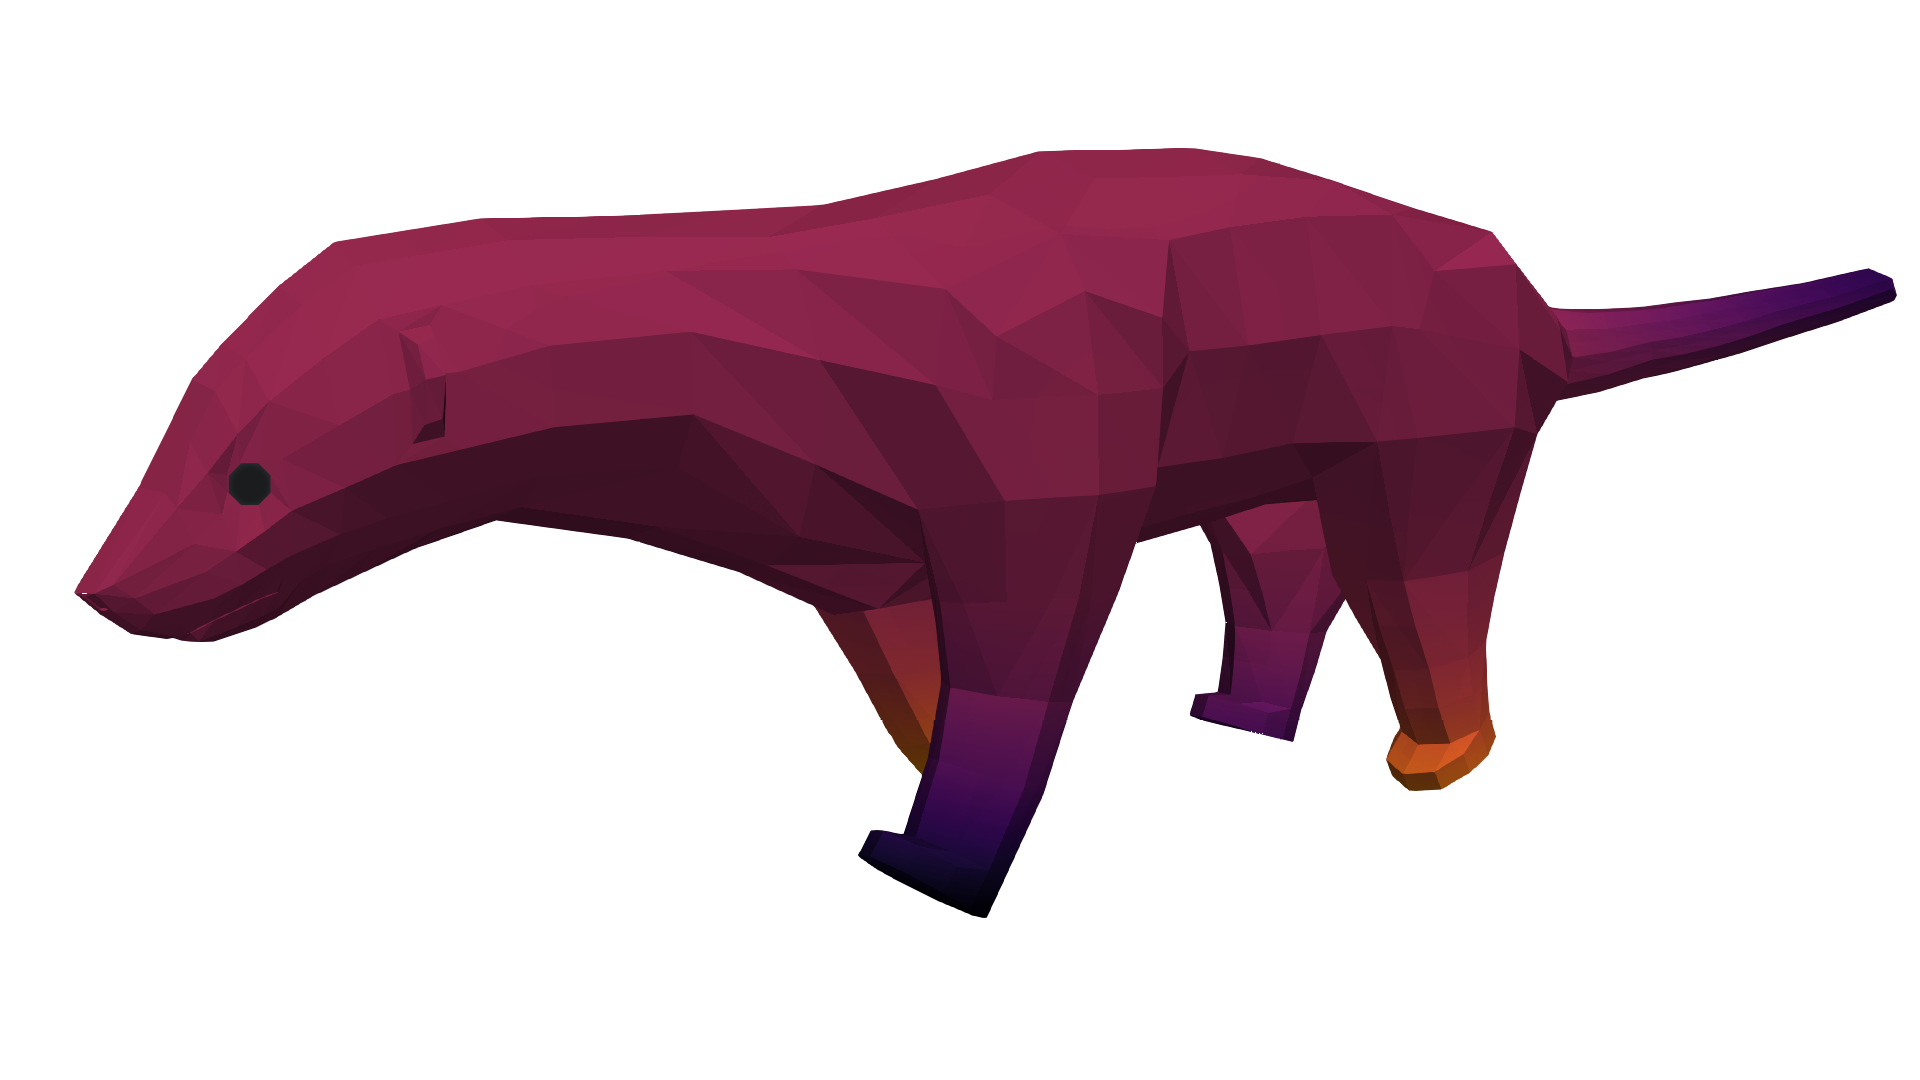
\includegraphics[height=2.75cm]{Ratellogo.png}
\end{center}

{\flushleft

Repository: https://gitlab.com/micromorph/ratel\\

~\\

Developers: Zach Atkins, Jed Brown, Leila Ghaffari,\\
\hspace{19mm} Rezgar Shakeri, Ren Stengel, Jeremy L Thompson\\

~\\

The authors acknowledge support by the Department of Energy, National Nuclear Security Administration, Predictive Science Academic Alliance Program (PSAAP) under Award Number DE-NA0003962.

}

\begin{center}

\includegraphics[height=0.7cm]{psaap-center-logos}
\end{center}

\end{frame}

%------------------------------------------------

\begin{frame}
\begin{center}
\frametitle{Overview}

Ratel - high order, performance portable solid mechanics\\

~\\

Built on libCEED and PETSc\\

~\\

GPU and CPU performance\\

~\\

\end{center}
\end{frame}
 
%------------------------------------------------

\begin{frame}
\frametitle{Overview} % Table of contents slide, comment this block out to remove it
\tableofcontents % Throughout your presentation, if you choose to use \section{} and \subsection{} commands, these will automatically be printed on this slide as an overview of your presentation
\end{frame}

%------------------------------------------------
\section{Background}
%------------------------------------------------

\begin{frame}
\begin{center}
\frametitle{ECP Roots}

\begin{itemize}

\item Ratel built directly on results from ECP CEED project\\

~\\

\item libCEED provides high-performance operator evaluation\\

~\\

\item PETSc provides linear/non-linear solvers and time steppers\\

~\\

\item Ratel built from libCEED + PETSc solid mechanics demo app\\

\end{itemize}

\end{center}
\end{frame}

%-------------------------------------------------------------------------------

\begin{frame}
\begin{center}
\frametitle{Modern Hardware}

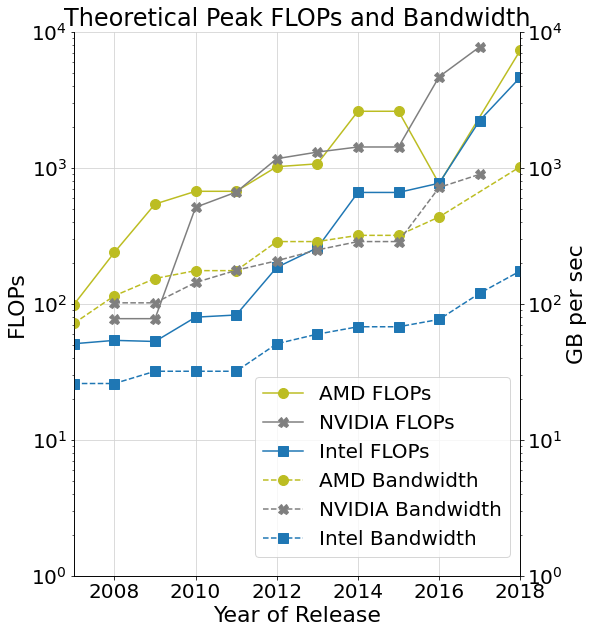
\includegraphics[height=5.5cm]{peakFlopsAndBandwidth_tall}
\hspace{1cm}
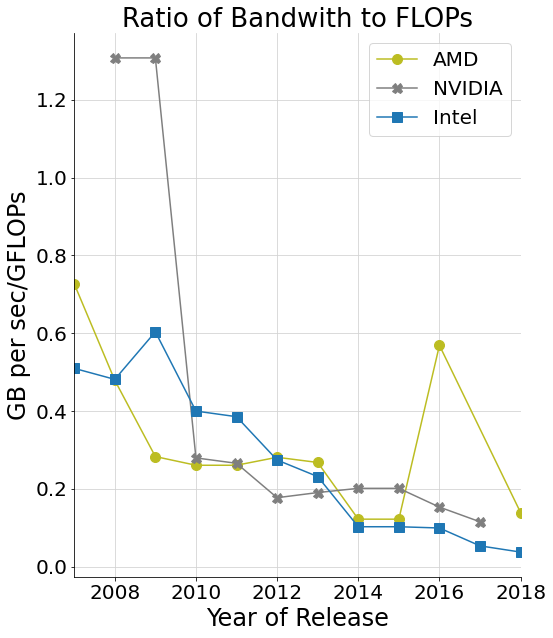
\includegraphics[height=5.5cm]{peakRatio_tall}

Modern hardware has lower memory bandwidth than FLOPs

\end{center}
\end{frame}

%-------------------------------------------------------------------------------

\begin{frame}
\begin{center}
\frametitle{Benefits of Matrix-Free}

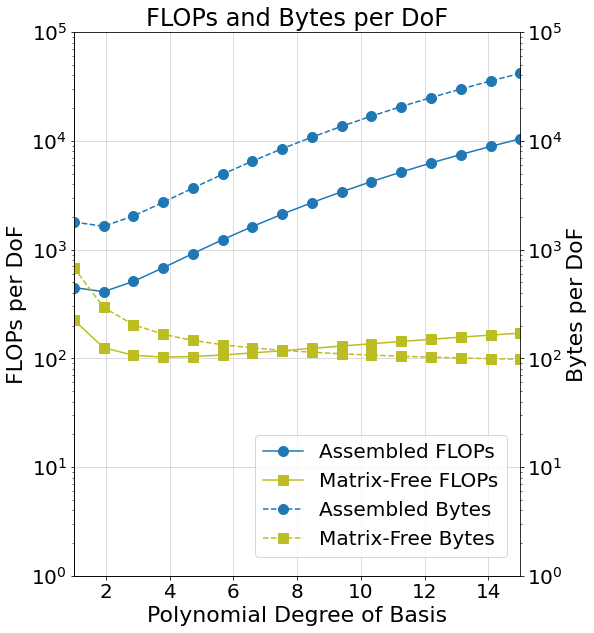
\includegraphics[height=5.5cm]{assembledVsMatrixFree_tall}
\hspace{1cm}
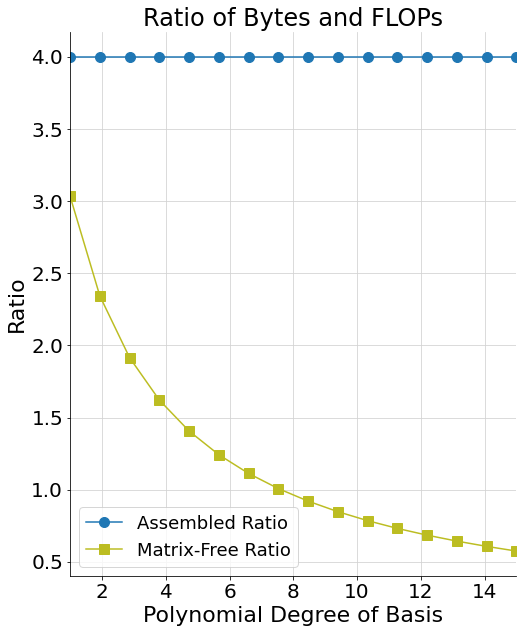
\includegraphics[height=5.5cm]{assembledVsMatrixFreeBalance_tall}

{\small Requirements for matrix-vector product with sparse matrix vs matrix-free\\ for screened Poisson $\nabla^2 u - \alpha^2 u = f$ in 3D}\\

{\bf Matrix-free representations using tensor product bases\\better match modern hardware limitations}

\end{center}
\end{frame}

%------------------------------------------------

\begin{frame}
\begin{center}
\frametitle{Matrix-Free Operators from libCEED}

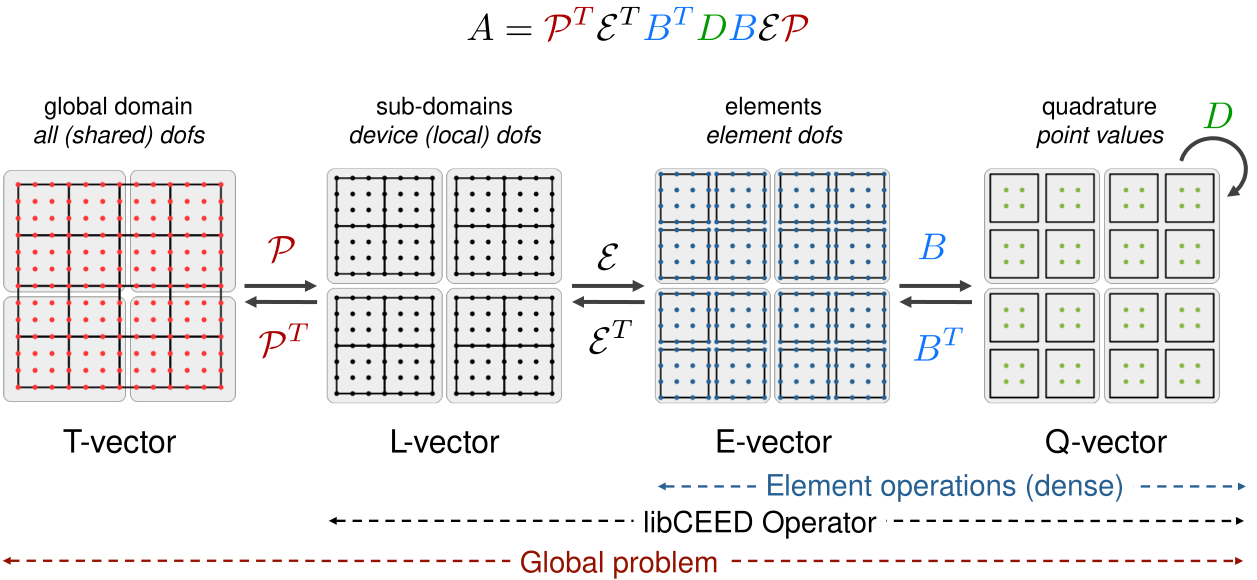
\includegraphics[height=5.0cm]{libCEEDAPI.png}

~\\

libCEED provides arbitrary order matrix-free operator evaluation\\

\end{center}
\end{frame}

%------------------------------------------------

\begin{frame}
\begin{center}
\frametitle{Performance Portability from libCEED}

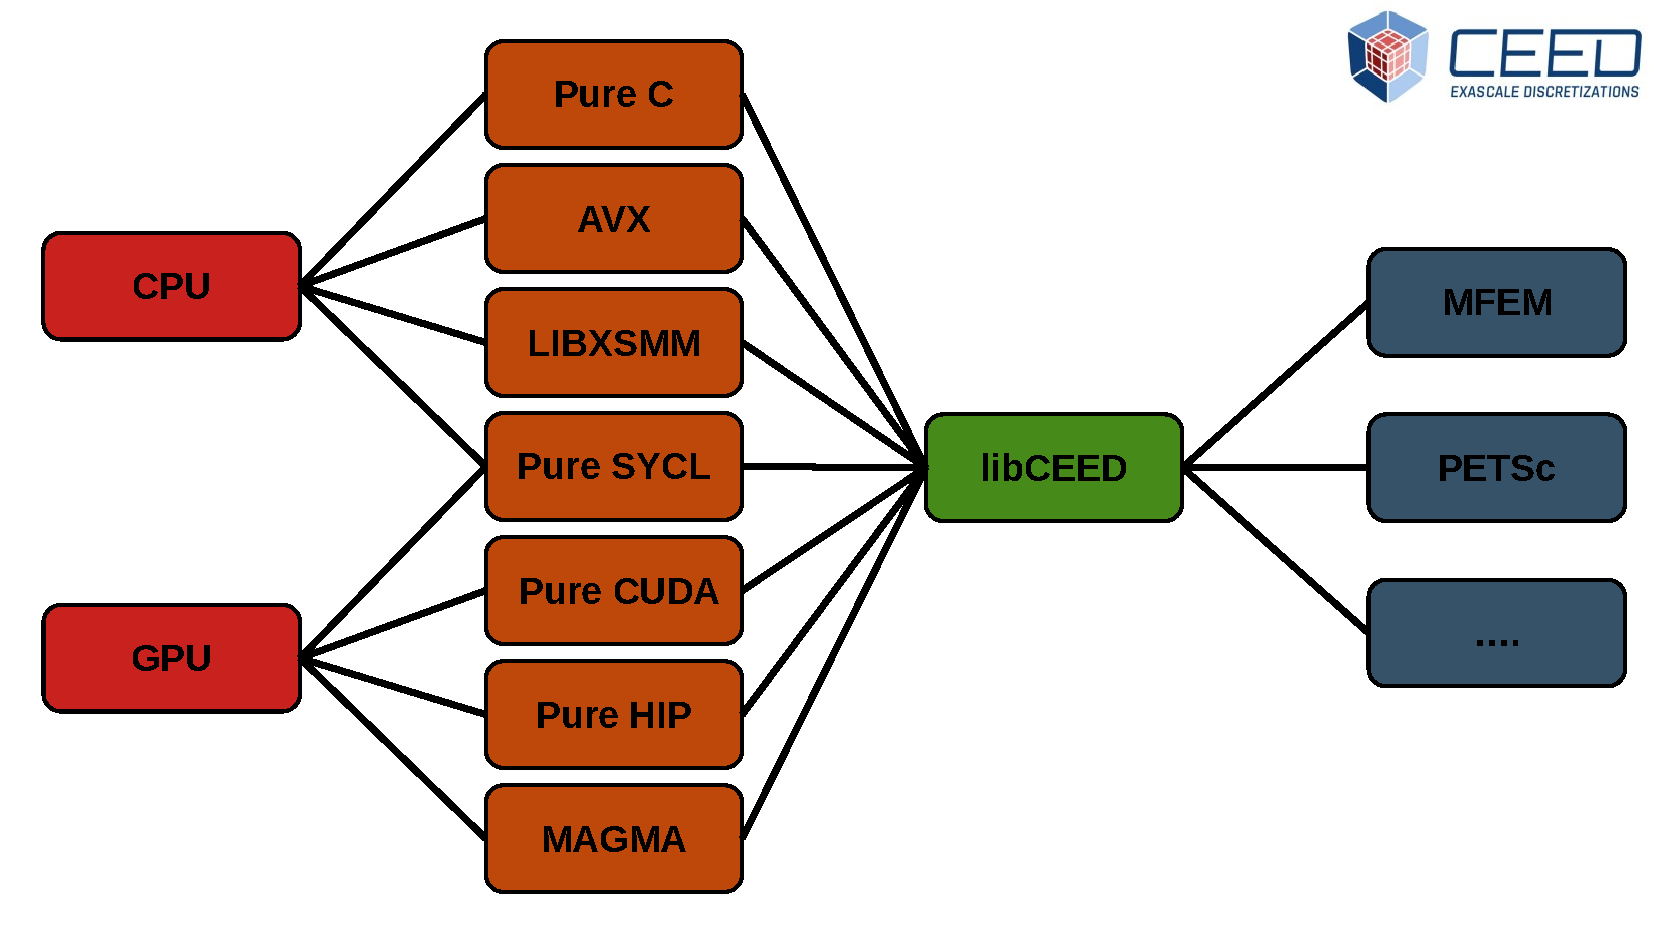
\includegraphics[height=5.5cm]{libCEEDBackends.pdf}

~\\

Performance portability with libCEED's matrix-free operators\\

\end{center}
\end{frame}

%------------------------------------------------

\begin{frame}
\begin{center}
\frametitle{Extensible Solvers from PETSc}

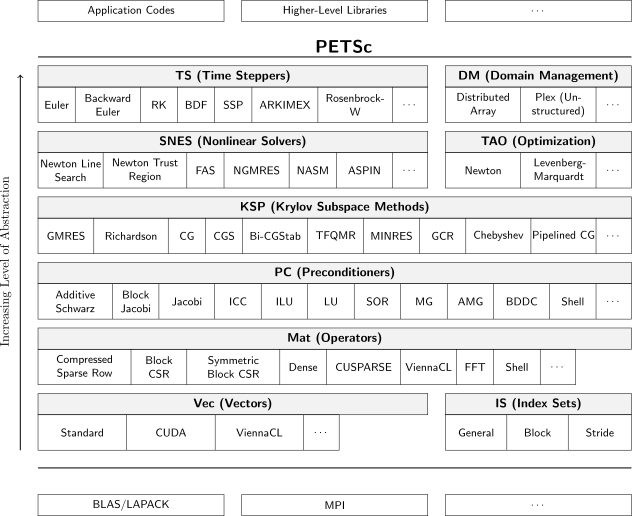
\includegraphics[height=6.0cm]{PETScAPI.png}

~\\

PETSc provides extensible, scalable solvers\\

\end{center}
\end{frame}

%------------------------------------------------
\section{Ratel Features}
%------------------------------------------------

\begin{frame}
\begin{center}
\frametitle{Ratel}

\begin{center}
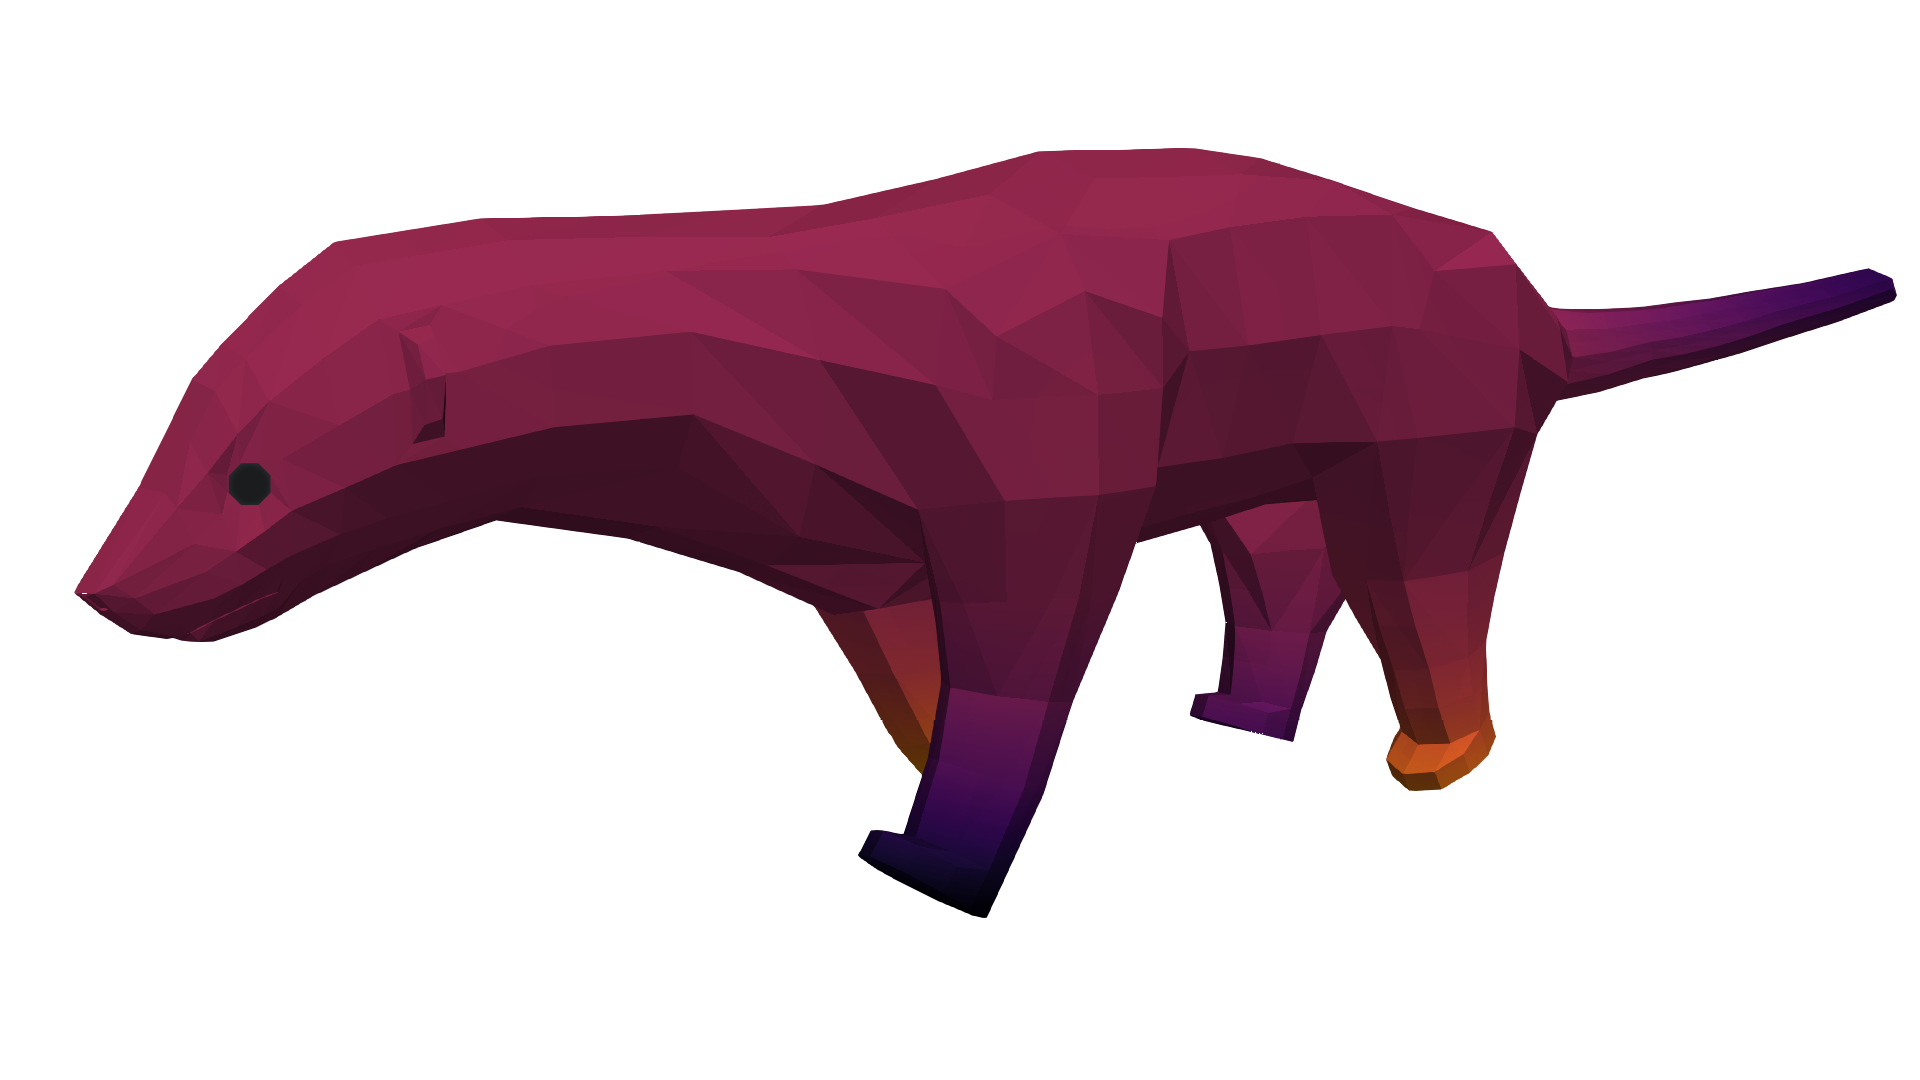
\includegraphics[height=2.5cm]{Ratellogo.png}
\end{center}

Ratel supports...

\begin{itemize}

\item hyperelastic and plastic material models

\item on unstructured meshes with multiple material regions

\item with arbitrary order mixed finite elements

\item using efficient matrix-free operator evaluation

\item with multiple solver and time-stepper options

\item and $p$-multigrid preconditioners using AMG course grid solves

\item on both CPU and GPU with runtime selection

\end{itemize}

\end{center}
\end{frame}

%------------------------------------------------

\begin{frame}
\begin{center}
\frametitle{Material Models}

Ratel supports several material models:\\

~\\

\begin{itemize}

\item Linear elasticity\\

\item Neo-Hookean hyperelasticity\\

\item Mooney-Rivlin hyperelasticity\\

\item Odgen hyperelasticity\\

\item Linear plasticity with linear hardening (further work ongoing)\\

\item Linear elasticity with AT2 damage model (in testing)\\

\item CEED benchmark problems\\

\item more in development...\\

\end{itemize}

\end{center}
\end{frame}

%-------------------------------------------------------------------------------

\begin{frame}[fragile]
\begin{center}
\frametitle{Material Model Specification}

{\footnotesize
\begin{lstlisting}[style=yaml]
dm_plex:
  filename: examples/meshes/rod-and-binder.msh
  simplex: 0

material: rod,binder

binder: 
  model: elasticity-neo-hookean-initial
  E: 2.
  nu: 0.4
  label_value: 4

rod:
  model: elasticity-mooney-rivlin-initial
  mu_1: 0.5
  mu_2: 0.5
  nu: 0.4
  label_value: 3
\end{lstlisting}
}

\end{center}
\end{frame}

%------------------------------------------------

\begin{frame}
\begin{center}
\frametitle{Additional Material Models}

Many material models support several options:\\

~\\

\begin{itemize}

\item Initial configuration\\

\item Current configuration\\

\item Automatic differentiation (Enzyme)\\

\item Isochoric formulation\\

\item Mixed FEM (displacement, pressure split, incompressible materials)\\

\end{itemize}

\end{center}
\end{frame}

%------------------------------------------------

\begin{frame}
\begin{center}
\frametitle{Boundary Conditions}

Ratel supports various boundary conditions:\\

~\\

\begin{itemize}

\item Time varying Dirichlet clamp\\

\item Time varying Dirichlet slip\\

\item Time varying traction\\

\item Pressure loading due to liquid or gas contact\\

\item Nitsche's method solid contact with Coulomb friction\\

\end{itemize}

\end{center}
\end{frame}

%-------------------------------------------------------------------------------

\begin{frame}[fragile]
\begin{center}
\frametitle{Boundary Condition Specification}

{\footnotesize
\begin{lstlisting}[style=yaml]
bc:
  clamp: 5
  clamp_5_translate: -0.2,0,0, 0,0,0, .2,0,0
  clamp_5_rotate: 1,0,0,.2,0, 1,0,0,0,0, 1,0,0,-.2,0,
  clamp_5_times: 0.33, 0.66, 1.0
  clamp_5_interpolation: linear

  platen: 6
  platen_6:
    normal: -1,0,0
    center: 1.0,0.5,0.5
    distance: 0.2
    gamma: 1000
\end{lstlisting}
}

\end{center}
\end{frame}

%------------------------------------------------

\begin{frame}
\begin{center}
\frametitle{Solver Modes}

Three sample applications are provided:\\

~\\

\begin{itemize}

\item Static Elasticity\\

~\\

\item Quasi-static Elasticity\\

~\\

\item Dynamic Elasticity\\

\end{itemize}

~\\

all using $p$-multigrid + coarse grid AMG by default

\end{center}
\end{frame}

%------------------------------------------------
\section{iMPM Development Progress}
%------------------------------------------------

\begin{frame}
\begin{center}
\frametitle{What is MPM?}

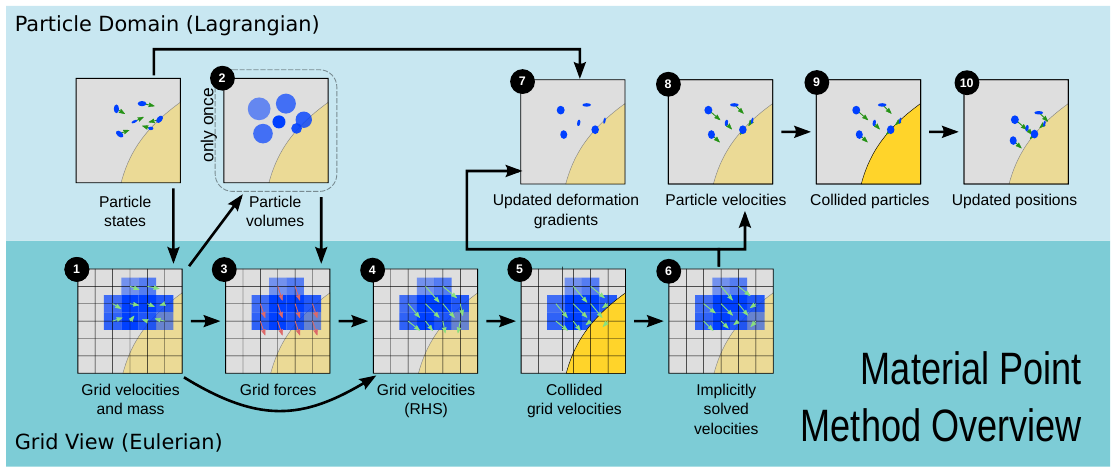
\includegraphics[height=5cm]{MPMOverview.png}\\

~\\

\begin{itemize}

\item Continuum based partical method with background mesh for gradients\\

\item Extension of FLIP (which is an extension of PIC)\\

\item Used in rendering for the movie \emph{Frozen}\\

\end{itemize}

\end{center}
\end{frame}

%------------------------------------------------

\begin{frame}
\begin{center}
\frametitle{What does MPM have to do with FEM?}

\begin{itemize}

\item Problem on background mesh changes when material points move\\

~\\

\item Natural fit for matrix-free representation\\

~\\

\item Similar reasoning to use matrix-free for adaptive methods\\

~\\

\item Ratel FEM infrastructure provides fast background mesh solves\\

\end{itemize}

\end{center}
\end{frame}

%------------------------------------------------

\begin{frame}
\begin{center}
\frametitle{libCEED Basis Evaluation to Points}

\begin{center}
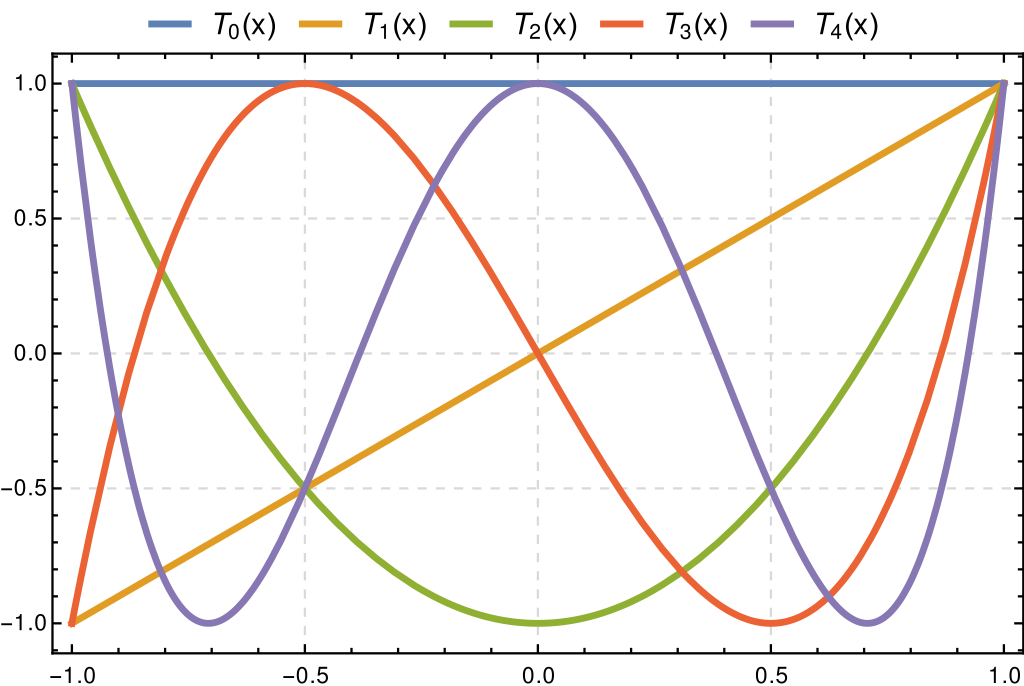
\includegraphics[height=4cm]{ChebyshevPolynomials.png}
\end{center}

\begin{itemize}

\item Interpolate from primal to dual (quadrature) space\\

\item Fit Chebyshev polynomials to values at quadrature points\\

\item Evaluate Chebyshev polynomials at reference coords of material points\\

\item Transpose the order for projection to mesh from material points\\

\end{itemize}

\end{center}
\end{frame}

%------------------------------------------------

\begin{frame}
\begin{center}
\frametitle{DMSwarm for Material Points}

\begin{center}
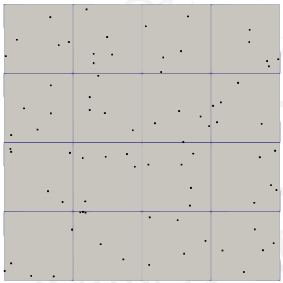
\includegraphics[height=4cm]{DMSwarmOverview.png}
\end{center}

\begin{itemize}

\item PETSc DMSwarm manages material points\\

~\\

\item PETSc DMPlex manages cells (elements)\\

~\\

\item Exposing API for cell reference coordinates of points\\

\end{itemize}

\end{center}
\end{frame}

%------------------------------------------------

\begin{frame}
\begin{center}
\frametitle{Current Work}

\begin{center}
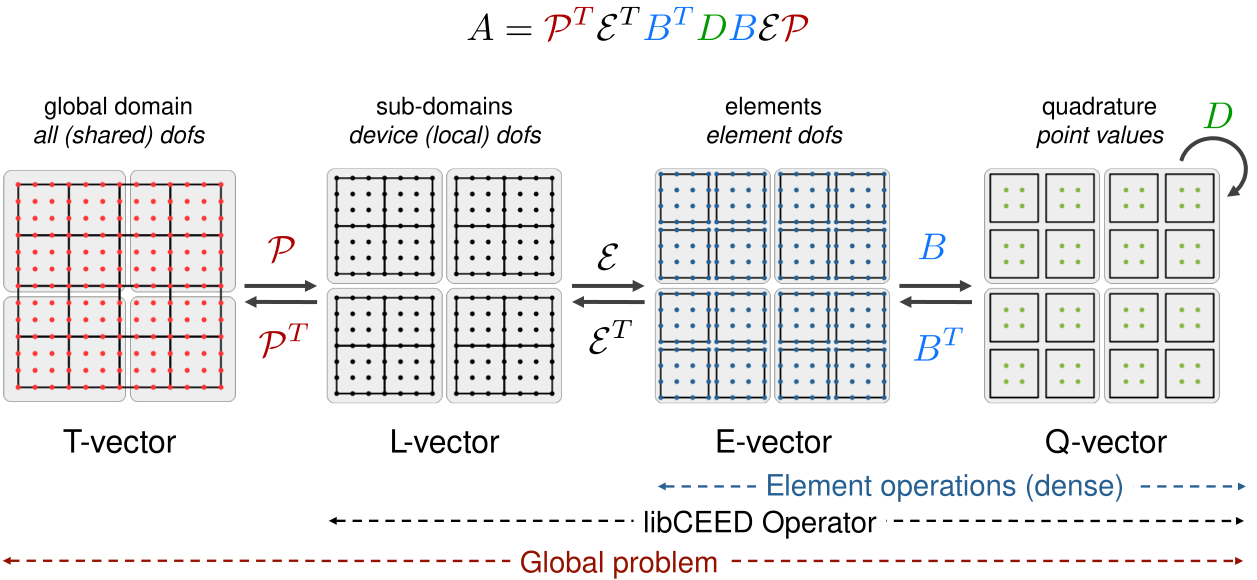
\includegraphics[height=5.0cm]{libCEEDAPI.png}
\end{center}

~\\

Building the libCEED element restriction operation for material points\\

~\\

Also need CeedOperator API to support evaluation at material points\\

\end{center}
\end{frame}

%------------------------------------------------
\section{Future Work}
%------------------------------------------------

\begin{frame}
\begin{center}
\frametitle{Future Work}

\begin{itemize}

\item Continued iMPM development\\

\item Addition of fluid dynamics models\\

\item PCPMG and PCFIELDSPLIT integration\\

\item Upstream PETSc + libCEED integration\\

\item Python and Rust interfaces\\

\item User model interface in C and Rust\\

\item We invite contributors and friendly users\\

\end{itemize}

\end{center}
\end{frame}
 
%------------------------------------------------

\begin{frame}
\frametitle{Questions?}

\begin{center}
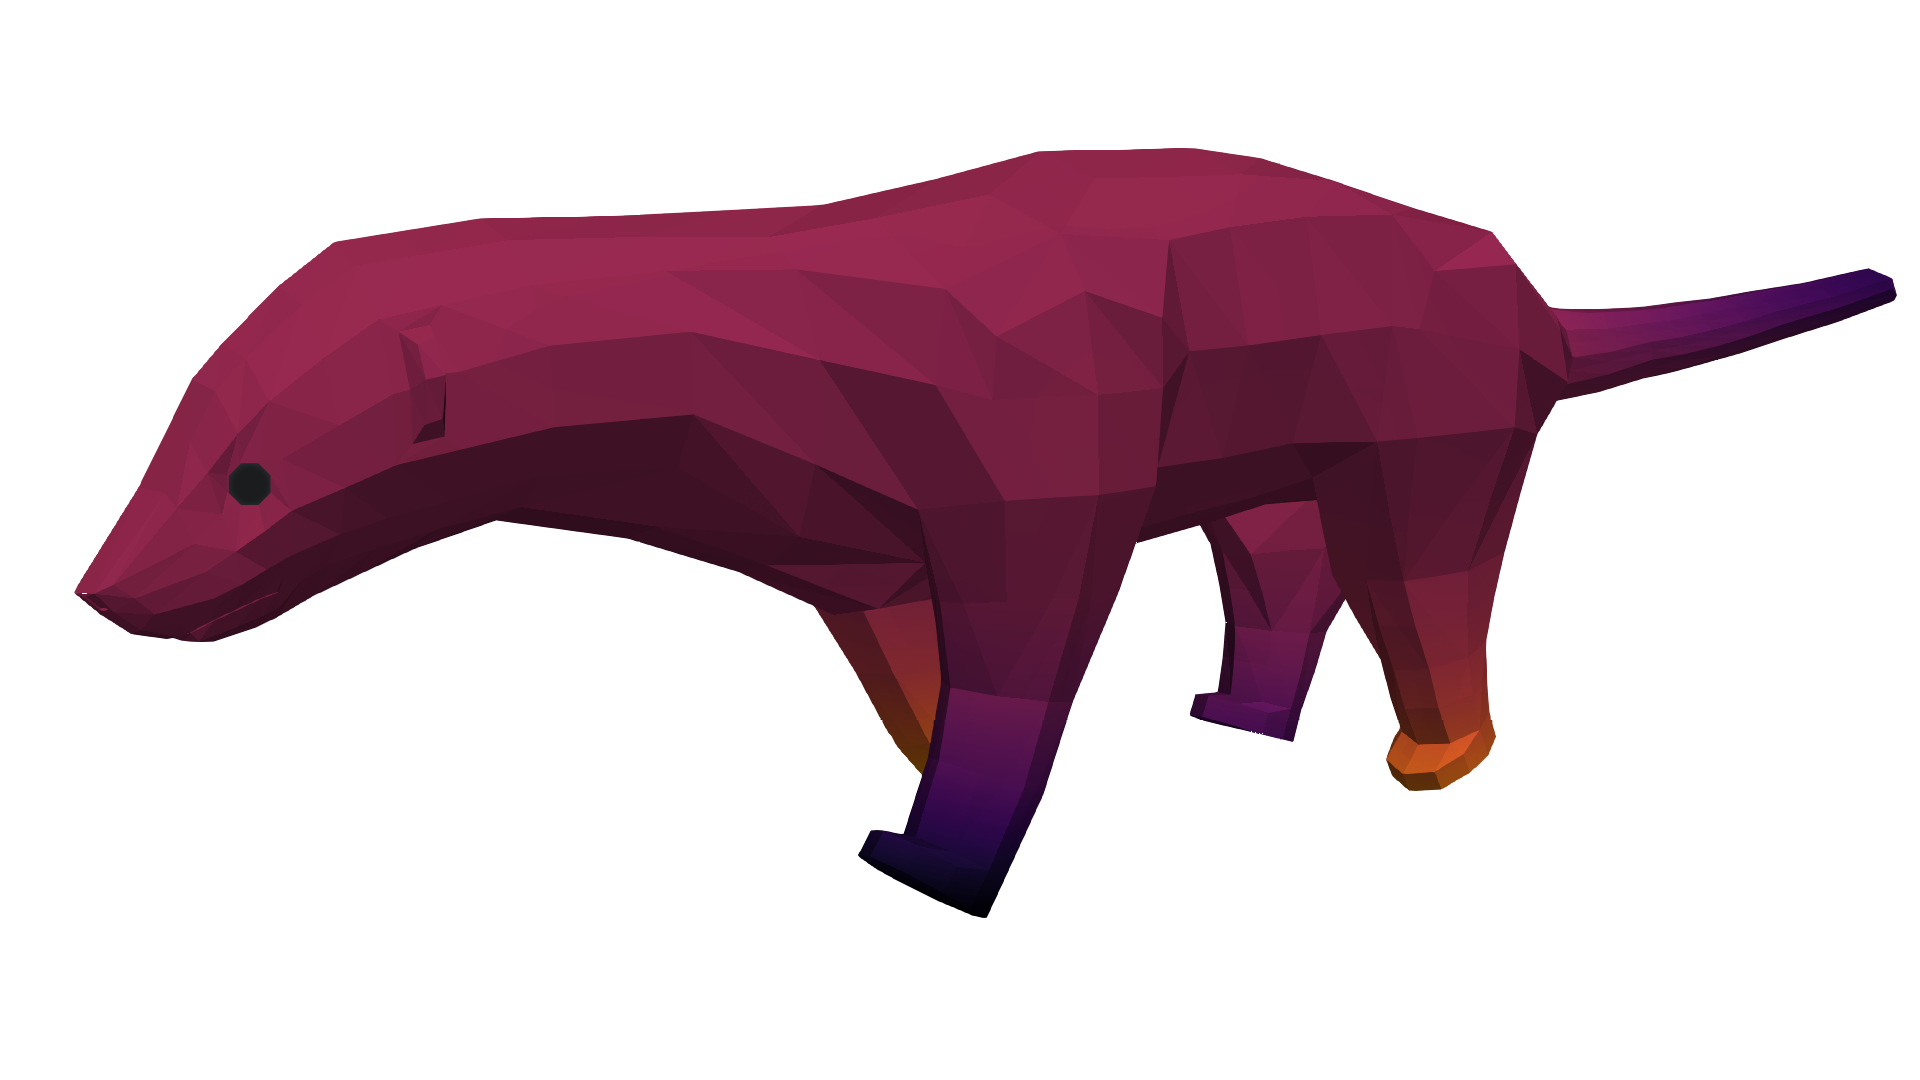
\includegraphics[height=2.75cm]{Ratellogo.png}
\end{center}

{\flushleft

Repository: https://gitlab.com/micromorph/ratel\\

~\\

Ratel Team: Zach Atkins, Jed Brown, Leila Ghaffari,\\
\hspace{19mm} Rezgar Shakeri, Ren Stengel, Jeremy L Thompson\\

~\\

Grant: Predictive Science Academic Alliance Program (DE-NA0003962)\\

}

\begin{center}

\includegraphics[height=0.8cm]{psaap-center-logos}
\end{center}

\end{frame}

%-------------------------------------------------------------------------------

\end{document}

%-------------------------------------------------------------------------------
